
\documentclass[11pt]{article}
\usepackage{amsmath,amssymb,amsfonts} 
\usepackage{epsfig} \usepackage{latexsym,nicefrac,bbm}
\usepackage{xspace}
\usepackage{color,fancybox,graphicx,subfigure,fullpage}
\usepackage[top=1.25in, bottom=1.25in, left=1in, right=1in]{geometry}
\usepackage{tabularx} \usepackage{hyperref} 
\usepackage{pdfsync}
\usepackage[boxruled]{algorithm2e}
\usepackage{multicol}
\usepackage{enumitem}
\newcommand{\parag}[1]{ {\bf \noindent #1}}
\newcommand{\defeq}{\stackrel{\textup{def}}{=}}
\newcommand{\nfrac}{\nicefrac}
\newcommand{\opt}{\mathrm{opt}}
\newcommand{\tO}{\widetilde{O}}
\newcommand{\polylog}{\mathop{\mbox{polylog}}}
\newcommand{\supp}{\mathrm{supp}}
\newcommand{\rank}{\mathrm{rank}}
\newcommand{\ptot}{p_{\mathrm{tot}}}
\newcommand{\pmin}{p_{\mathrm{min}}}
\newcommand{\pmax}{p_{\mathrm{max}}}
\newcommand{\prob}[1]{\mathrm{Pr}\insquare{#1}}


\newcommand{\conv}{\mathrm{conv}}
\newcommand{\dist}{\mathrm{dist}}
\newcommand{\argmin}{\operatornamewithlimits{argmin}}
\newcommand{\sgn}{\mathrm{sgn}}
\newcommand{\fc}{\mathrm{fc}}


\newcommand{\cM}{\mathcal{M}}
\newcommand{\cB}{\mathcal{B}}
\newcommand{\cU}{\mathcal{U}}
\newcommand{\cY}{\mathcal{Y}}
\newcommand{\cF}{\mathcal{F}}
\newcommand{\capa}{\mathrm{Cap}}
\newcommand{\dcapa}{\underline{\mathrm{Cap}}}
\newcommand{\st}{\mathrm{s.t.}}
\newcommand{\un}{\mathrm{un}}

\newcommand{\Pb}{\mathbb{P}}
\newcommand{\sym}{\mathrm{sym}}
\newcommand{\pcount}{\mathbf{PCount}}
\newcommand{\mixdet}{\mathbf{MixDisc}}
\newcommand{\sbold}{\mathbf{S}}
\newcommand{\mb}{{M(\cB)}}

\newcommand{\mlb}{{M_{\mathrm{lin}}(\cB)}}
\newcommand{\redc}[1]{ \textcolor{red} {#1}}
\newcommand{\newt}{\mathrm{Newt}}
\newcommand{\wtf}{\widetilde{f}}
\newcommand{\wt}{\widetilde}
\newcommand{\diam}{\mathrm{diam}}
\newcommand{\lspan}{\mathrm{span}}
\newcommand{\interior}{\mathrm{int}}
\newcommand{\aff}{\mathrm{aff}}
\newcommand{\per}{\mathrm{per}}
\newcommand{\bl}{\mathrm{BL}}
\newcommand{\cE}{\mathbb{E}}


\newcommand{\eps}{\varepsilon}

\newenvironment{proof}{\noindent{\bf Proof:}\hspace*{1em}}{\qed\bigskip}
\clubpenalty=10000
\widowpenalty = 10000
\newcommand{\qed}{\hfill\ensuremath{\square}}


\def\showauthornotes{0} 
\def\showkeys{0} 
\def\showdraftbox{0}


\newcommand{\Snote}{\Authornote{S}}
\newcommand{\Scomment}{\Authorcomment{S}}

\newcommand\Z{\mathbb Z}
\newcommand\N{\mathbb N}
\newcommand\R{\mathbb R}
\newcommand\C{\mathbb C}

\newtheorem{theorem}{Theorem}[section]
\newtheorem{fact}{Fact}[section]
\newtheorem{conjecture}[theorem]{Conjecture}
\newtheorem{definition}{Definition}[section]
\newtheorem{lemma}[theorem]{Lemma}
\newtheorem{remark}[theorem]{Remark}
\newtheorem{proposition}[theorem]{Proposition}
\newtheorem{corollary}{Corollary}[section]
\newtheorem{claim}[theorem]{Claim}

\newtheorem{openprob}[theorem]{Open Problem}
\newtheorem{remk}[theorem]{Remark}
\newtheorem{example}[theorem]{Example}
\newtheorem{apdxlemma}{Lemma}
%\newtheorem{algorithm}[theorem]{Algorithm}
\newcommand{\question}[1]{{\sf [#1]\marginpar{?}} }

%% probability stuff

\newcommand\pr{\mathop{\mbox{\bf Pr}}}
\newcommand\av{\mathop{\mbox{\bf E}}}
\newcommand\var{\mathop{\mbox{\bf Var}}}

\newcommand{\ex}[1]{\av\left[{#1}\right]}
\newcommand{\Ex}[2]{\av_{{#1}}\left[{#2}\right]}

\def\abs#1{\left| #1 \right|}
\newcommand{\norm}[1]{\ensuremath{\left\lVert #1 \right\rVert}}



\newcommand{\tr}[1]{\mathop{\mbox{Tr}}\left({#1}\right)}
\newcommand{\diag}[1]{{\sf Diag}\left({#1}\right)}

\newcommand\set[1]{\left\{#1\right\}} %usage \set{1,2,3,,}
\newcommand{\poly}{\mathrm{poly}}
\newcommand{\floor}[1]{\left\lfloor\, {#1}\,\right\rfloor}
\newcommand{\ceil}[1]{\left\lceil\, {#1}\,\right\rceil}
\newcommand{\comp}[1]{\overline{#1}}
\newcommand{\pair}[1]{\left\langle{#1}\right\rangle} %for inner product
\newcommand{\smallpair}[1]{\langle{#1}\rangle}

\newcommand{\inparen}[1]{\left(#1\right)}             %\inparen{x+y}  is (x+y)
\newcommand{\inbraces}[1]{\left\{#1\right\}}           %\inbrace{x+y}  is {x+y}
\newcommand{\insquare}[1]{\left[#1\right]}             %\insquare{x+y}  is [x+y]
\newcommand{\inangle}[1]{\left\langle#1\right\rangle} %\inangle{A}    is <A>


\newenvironment{proofsketch}{\begin{trivlist} \item {\bf
Proof Sketch:~~}}
  {\qedsketch\end{trivlist}}

\newenvironment{proofof}[1]{\begin{trivlist} \item {\bf Proof
#1:~~}}
  {\qed\end{trivlist}}


\title{\bf Modeling Alternative Affordable Housing Priority Systems }


\author{ Andrew West, Nicole Lam, Atul Pokharel, Urszula Solarz  \\ \\ 
Course: CPSC 464 \\ 
Professor: Nisheeth K. Vishnoi
}




\begin{document}


\maketitle
 
%\begin{abstract}
%
%Write a 6-8 line abstract clearly stating the high level goals and the concrete desired goals of this project. 
%  
%\end{abstract}
%
%
%\newpage
%
%
%
%%\tableofcontents
%
%\newpage

\section{Proposal}

\paragraph{High level description of the problem.}

We propose to empirically examine how biases in housing allocation compound in queues that permit choice. More generally, we propose to study the fairness properties of housing allocation schemes that do and do not permit choice on the part of recipients.

 
\paragraph{Motivation to study the problem and its importance.}
Housing is a basic necessity that is in increasingly scarce supply in American cities. Although the specific algorithms used to allocate affordable housing are not available, there appear to be two types based on whether or not the applicant is given any choice in the allocation. For example, after they are selected for housing by a lottery system, they may be presented with one or more options to choose from. 
Better understanding how the presence of this choice can mitigate or exacerbate biases could help public housing authorities assess the fairness of allocation schemes currently in use, as well as enable citizens to hold governments responsible for fair allocations of a scarce, basic resource.  \\
\newline
In general, there are two main modes of allocating housing to those who want it. One is the market mechanism in which those who can pay market price of housing receive it. A second one is through public housing agencies or similar non-market modes in which the cost of housing is significantly subsidized below market price. When there are fewer housing units than the number of those who want it and price cannot be used to allocate, who receives housing depends on an allocation algorithm. Some common algorithms for allocating housing in this latter scenario are lotteries and waitlists, with or without some other group-based preference ranking applied to it.   \\
\newline
There are two variations of non-market allocation algorithms depending on how much choice the recipient has. In the first, the recipient is presented with a choice of one or more units. They can either choose from among the set or choose to go back into the waitlist or lottery. While the fairness properties of different allocation schemes have been examined, to our knowledge, the fairness properties of allowing individuals to choose whether to accept or not is relatively understudied particularly in the presence of bias. 

\begin{figure}
    \centering
    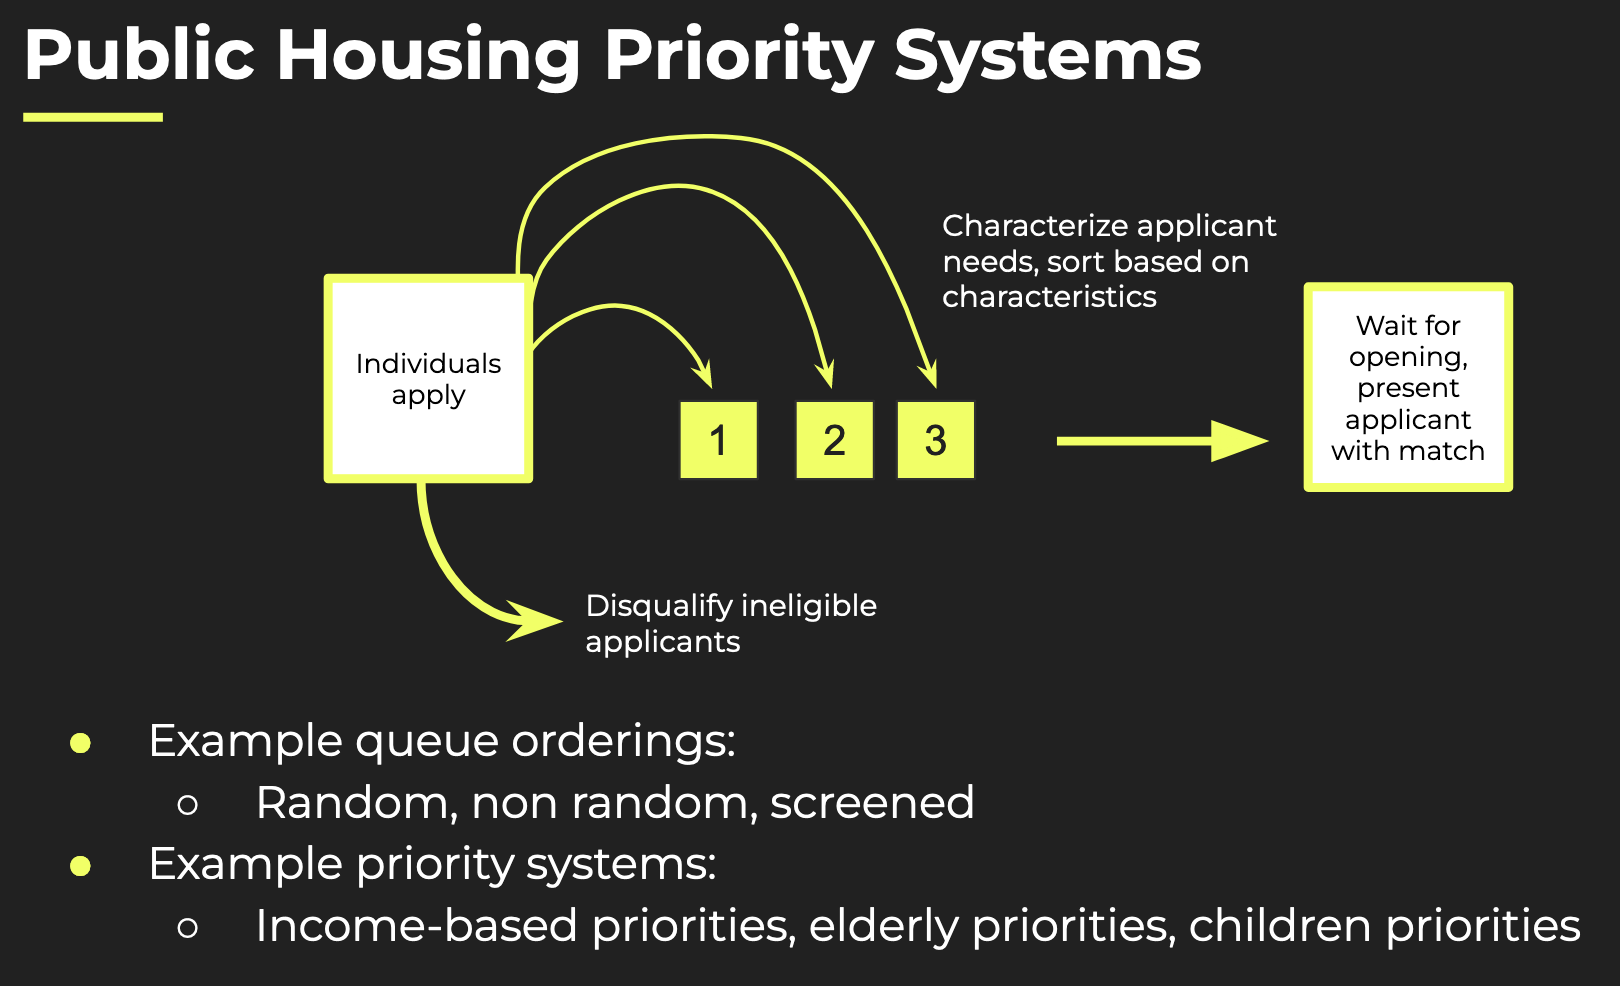
\includegraphics[width=0.75\linewidth]{schematic_priority _systems.png}
    \caption{Diagram of public housing allocation systems}
    \label{fig:schematic}
\end{figure}

\paragraph{Most related prior works.}
There are a variety of studies regarding affordable housing and approximating allocation algorithms. The major limitation of all these studies is that the algorithms are not public. However, Figure 1 describes the general stages of any scheme.\\
\newline
The allocation of scarce resources is a classic problem. There are papers abstracting the housing allocation problem into that of designing wait lists and lotteries \cite{arnosti2020design}. They examine in great detail those two modes of allocation, but do not examine the role of choice. From an even higher-level, others have examined the fairness trade-offs of different allocations of social services \cite{mashiat2022trade}. This provides a general analysis of the trade-offs, but do not give a way to assess the allocation mechanisms we have in mind.  \\
\newline
For our most related prior works, we examine two more specific papers that directly analyze, modify, or propose algorithms for housing allocation. \\
\newline
Our first paper tackles the issue that housing allocation methods are often unknown and opaque. Thus, they created an algorithm to include priority systems (moving populations with certain characteristics to the front of a queue) \cite{nyuaffordablehousing}. Specifically, they analyzed the changes in tenant composition after implementing priority for high income households, low income households, the elderly population, and families with children under 18. While the model sheds light on the magnitude of change in results for each priority system, it lacks significant key variables in their dataset (such as military status) and limits the eligible applicants to those whose household income is above 80\% of the area median income. We are also interested in exploring the nuances of implementing an overlap of different priority systems, while this paper only does each individually.\\
\newline
In another paper, the author addresses a related issue to the housing allocation system: its inefficiency \cite{harvardpublichousing}. Most housing systems allow accepted applicants to reject the housing they are assigned, creating stretches of vacant buildings before they are re-entered in the system. The author then proposes a system where applicants choose to join the waitlist for one specific building type, allowing applicants to trade off their preferences for different units versus wait time. The paper only observes the issue of housing from a “demand” perspective; thus, the algorithm ignores inefficiencies in the system when the rate of building vacancies decrease.
\paragraph{Desired contributions.}
Figure 2 shows the main tasks and contributions.
\begin{figure}
    \centering
    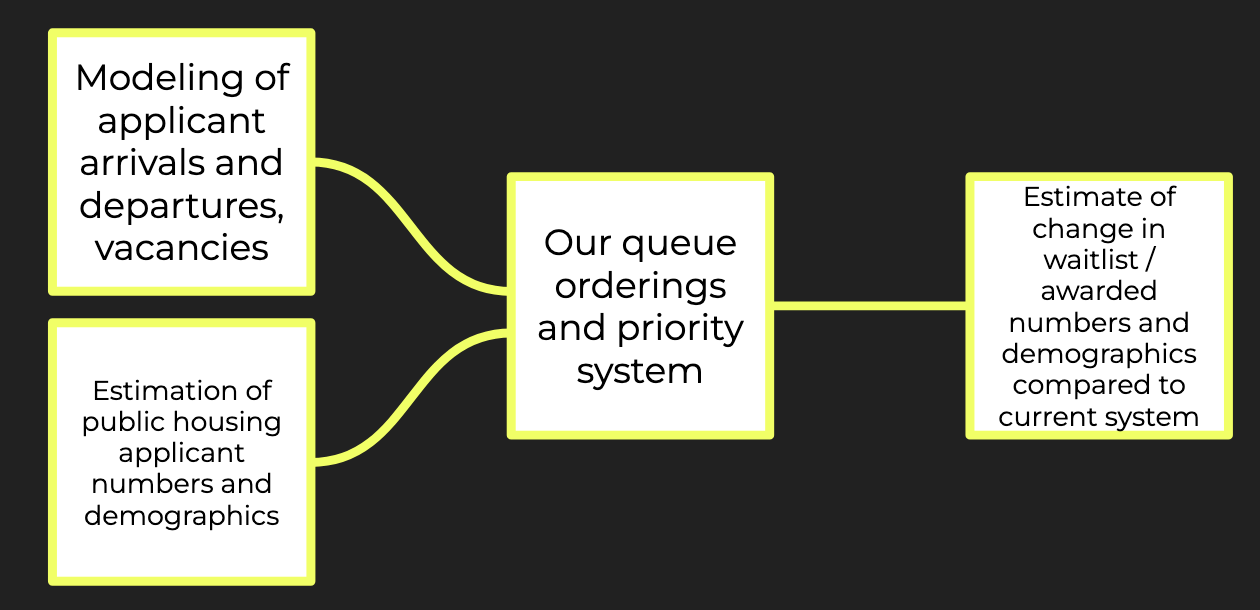
\includegraphics[width=0.75\linewidth]{ourmodel.png}
    \caption{Proposed model of our contributions}
    \label{fig:enter-label}
\end{figure}
Our work will be twofold: first, we aim to model the existing conditions of our chosen city's public housing allocation, followed by assessing new queue and priority systems and examining their effects on the demographics of those we predict will be offered public housing. \\
\newline
Little is typically known about the methods that cities use to allocate public housing, meaning our first task is to model this process. Using publicly available data on who is awarded housing, we can estimate this process for our chosen city. Relying on estimations made by previous works, we can also integrate assumptions about the rate at which housing becomes available into our predictions to gain a comprehensive approximation of overall public housing availability and allocation. We can apply this model to our city of choice to estimate the flow of applicants in, through, and our of public housing under the city's current system. \\
\newline
With an established model for the present conditions of a city, we can proceed to evaluate alternative allocation systems for fairness. We will apply these alternative systems to our model in order to comment on how the characteristics of tenants shift with the goal of informing future decision making in this sphere.

\begin{itemize} 

\item Conceptual novelty: we expect that ours will be one of the few empirical examinations of fairness implications of choice in housing allocation schemes.

\item Technical novelty: we expect that we will have to develop novel means of approximating allocation mechanisms.

%\item Novelty in proofs (leave blank if not done yet or not applicable)

\item Empirical/experimental component: We will evaluate these schemes on real world datasets if available and on simulated datasets, if necessary. We will also aim to visualize these differences. 

\end{itemize}


\paragraph{Feasibility and potential risks.} \\

\begin{itemize}
\item Availability of municipal data and actual algorithms
\item Technical feasibility of modeling choice (currently in communication with Daniel Waldinger at NYU about reproducibility standards of prior works)
\end{itemize}

\paragraph{}
Notedly, historic housing policy decisions play a large part in dictating the effectiveness of current policy efforts. Therefore, technical improvements and considerations of the societal implications of the algorithms used in these policies are only part of the process of ensuring fairer housing allocation. We hope this paper encourages broader and more thoughtful discussion on the usage of computer science in improving the lives of urban dwellers. \\


%\section{Other related works}
%
%\section{Preliminaries / Problem statement} 
%This should contain all the required mathematical notation and background necessary for anything to come after.
%
%\section{The model/framework}
%
%
%
%
%
%
%\section{(Desired) Theoretical results}
%
%
%\subsection{Preliminary results}
%
%
%\section{(Desired) Empirical results}
%
%\subsection{Setup}
%\paragraph{Datasets.}
%
%\paragraph{Algorithms.}
%
%\paragraph{Baselines and metrics.}
%
%
%
%\subsection{Preliminary results}
%
%
%\section{Conclusion, limitations, and future Work}
%Discuss the importance of the results, state the limitations, and point out avenues of future work/open problems.
%


\bibliographystyle{plain}
\bibliography{references} 


\end{document}
